% Template for ICIP-2015 paper; to be used with:
%          spconf.sty  - ICASSP/ICIP LaTeX style file, and
%          IEEEbib.bst - IEEE bibliography style file.
% --------------------------------------------------------------------------
\documentclass{article}
\usepackage{spconf,amsmath,graphicx}
\usepackage{listings}
\usepackage{float}
\usepackage{pythonhighlight}
% Example definitions.
% --------------------
\def\x{{\mathbf x}}
\def\L{{\cal L}}

% Title.
% ------
\title{Processamento Digital de Imagens - Trabalho 2}
%
% Single address.
% ---------------
\name{Bruna Medeiros da Silva - 16/0048711}
\address{UnB - FGA}
%
% For example:
% ------------
%\address{School\\
%	Department\\
%	Address}
%
% Two addresses (uncomment and modify for two-address case).
% ----------------------------------------------------------
%\twoauthors
%  {A. Author-one, B. Author-two\sthanks{Thanks to XYZ agency for funding.}}
%	{School A-B\\
%	Department A-B\\
%	Address A-B}
%  {C. Author-three, D. Author-four\sthanks{The fourth author performed the work
%	while at ...}}
%	{School C-D\\
%	Department C-D\\
%	Address C-D}
%
\begin{document}
%\ninept
%
\maketitle

%
\section{Questão 1}

\label{subsec:1_a}
O processo de especificação de histograma pode ser descrito em três passos:

\begin{enumerate}
	\item Encontrar o histograma da imagem, que mostra graficamente a a distribuição de níveis de cinza da imagem;
	\item Encontrar os valores $s_k$ da Função de Distribuição Acumulada (CDF - \textit{Cumulative Distribution Function}) da imagem;
	\item Encontrar os valores $z_k$ da CDF da função especificada;
	\item Fazer a equivalência entre os valores de s para z;
	\item utilizar a nova CDF obtida para gerar uma nova imagem equalizada com os valores dos pixels $s_k$ convertidos para $z_k$.
\end{enumerate}

\subsection*{1.a - Algoritmo de especificação de histograma}
\subsubsection*{Histograma}
A primeira parte do passo 1 foi implementada em python na função descrita no Código \ref{cod:hist}, reponsável pela geração do histograma da imagem original. Os valores obtidos podem ser chamados de $p_r(r)$.

\subsubsection*{Gerando a CDF da imagem}
Para gerar a CDF da imagem, foi utilizada a equação \ref{eq:cdf_pr}, que calcula a probabilidade de os pixels possuírem valores menores ou iguais a determinado valor dentro do intervalo de níveis de cinza da imagem.

\begin{equation}
	\label{eq:cdf_pr}
	s_k = \frac{(L - 1)}{MN}\sum_{j = 0}^{k} p_r(j)
\end{equation}

Onde $L$ é igual ao número de níveis de cinza disponíveis ($2^{n_bits}$), $MN$ é a quantidade de pixels que a imagem possui e $k$ é o nível de cinza para o qual estamos fazendo o cálculo e $p_r(j)$ é o valor de $j$ no histograma. 

\textbf{Obs.:} Se o histograma não estiver normalizado, ou seja, com os valores entre 0 e 1, não é necessário multiplicar por $L - 1$.

O algoritmo utilizado para chegar a esses valores está descrito no código \ref{cod:cdf_2d}

\subsubsection*{CDF da função especificada}
Gerar a CDF a partir de uma PDF (\textit{Probability Density Function}) é um processo ainda mais simples, visto que nós já temos a probabilidade de cada valor, precisando apenas somá-los aos anteriores para obter a CDF equivalente (Equação \ref{eq:cdf_pz}).


\begin{equation}
	\label{eq:cdf_pz}
	G(z) = \sum_{j = 0}^{z} p_z(j)
\end{equation}
%\vspace{-pt}

Onde $p_z(j)$ é a probabilidade de um pixel ter o valor $j$.

Esse processo está descrito no Código \ref{cod:cdf_pdf}.

\subsubsection*{Valores correspondentes $z = G^{-1}(s)$}

O Código \ref{cod:inv_t}, que abrange os itens 4 e 5, realiza todo o restante do processo de inversão. 

Para encontrar o valor $z = G^{-1}(s)$, precisamos encontrar o menor z para o qual $G(z)$ seja o mais próximo possível de $s_k$.
Fazendo isso para todos os valores de s, teremos o valor equivalente em z para todos os níveis de cinza presentes na imagem.

Depois disso, apenas aplicamos essa transformação nos pixels da imagem e, caso necessário, geramos os novos gráficos de histograma, PDF e/ou CDF para efeitos de comparação.

\subsection*{1.b - Mostrando os resultados}
\subsubsection*{a. Histograma da imagem original ($p_r(r)$)}

\label{sec:format}
\begin{figure}[H]
	\label{original_hist}
	\begin{minipage}[b]{1.0\linewidth}
		\centering
		\centerline{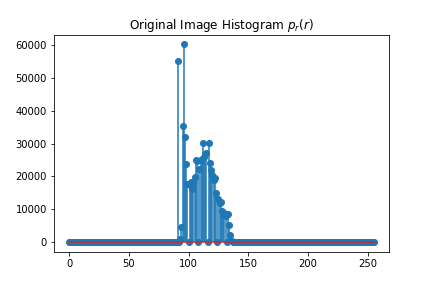
\includegraphics[width=8.5cm]{Figures/hist_original_fig}}
		%  \vspace{2.0cm}
		\centerline{Histograma da imagem original.}\medskip
	\end{minipage}
\end{figure}

\subsubsection*{b. Distribuição acumulada da função especificada ($G(z)$)}

\begin{figure}[H]
	\begin{minipage}[b]{1.0\linewidth}
		\label{fig:original_cdf}
		\centering
		\centerline{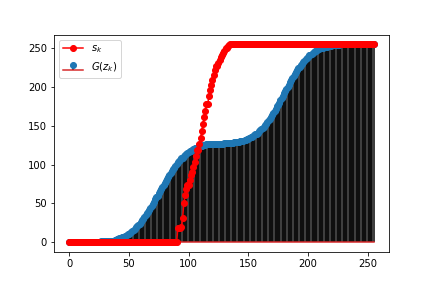
\includegraphics[width=8.5cm]{Figures/cdf_images}}
		%  \vspace{2.0cm}
		\centerline{CDF do histograma original ($s_k$) e da função especificada ($G(z)$).}\medskip
	\end{minipage}
\end{figure}

\subsubsection*{c. Gráfico da transformação inversa ($z = G^{-1}(s)$)}

\begin{figure}[H]
	\label{fig:t_graph}
	\begin{minipage}[b]{1.0\linewidth}
		\centering
		\centerline{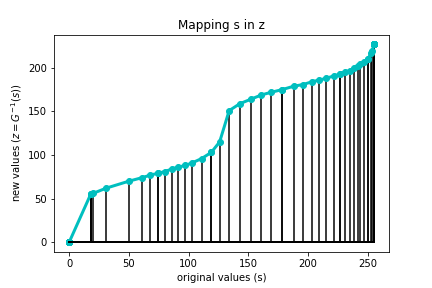
\includegraphics[width=8.5cm]{Figures/transform_graph}}
		%  \vspace{2.0cm}
		\centerline{Gráfico da Transformação Inversa ($z = G^{-1}(s)$).}\medskip
	\end{minipage}
\end{figure}

\subsubsection*{d. Histograma da imagem transformada}

\begin{figure}[H]
	\label{fig:t_hist}
	\begin{minipage}[b]{1.0\linewidth}
		\centering
		\centerline{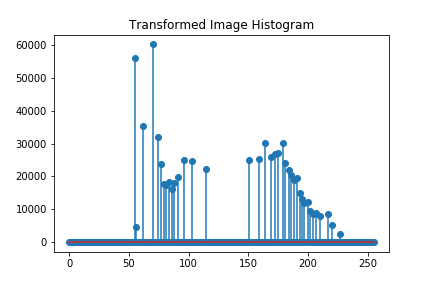
\includegraphics[width=8.5cm]{Figures/transformed_hist}}
		%  \vspace{2.0cm}
		\centerline{Histograma da Imagem transformada}\medskip
	\end{minipage}
\end{figure}

\begin{figure}[H]
	\label{fig:cdf}
	\begin{minipage}[b]{1.0\linewidth}
		\centering
		\centerline{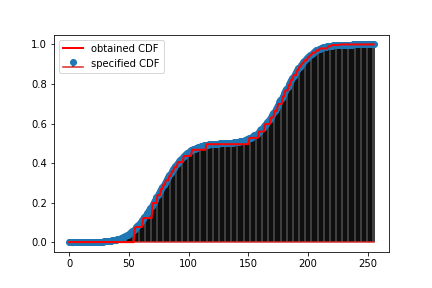
\includegraphics[width=8.5cm]{Figures/transformed_cdf}}
		%  \vspace{2.0cm}
		\centerline{Comparação entre CDF obtido e CDF da função especificada}\medskip
	\end{minipage}
\end{figure}

Para finalizar, temos as imagens original e resultante para análise dos resultados na Figura \ref{fig:img1}.

\begin{figure}[H]
	\label{fig:img1}
	\begin{minipage}[b]{1.0\linewidth}
		\centering
		\centerline{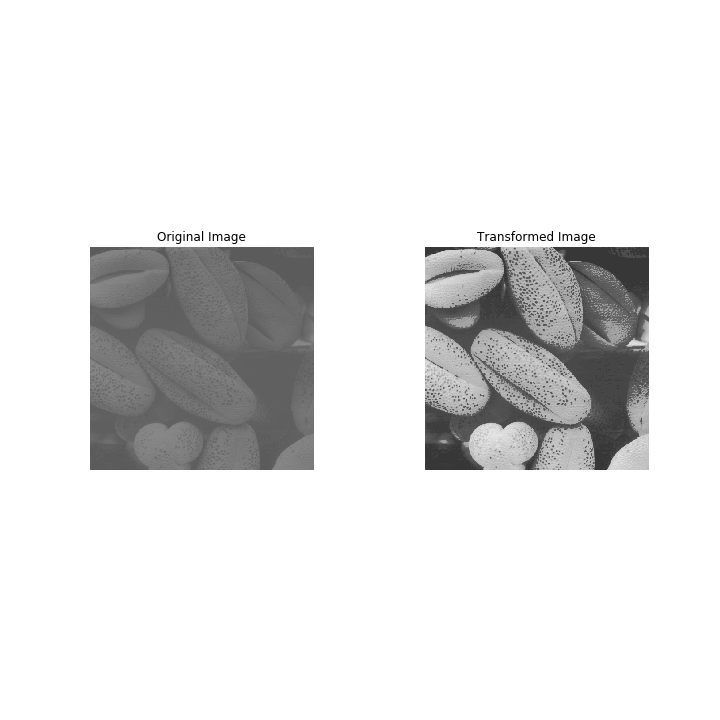
\includegraphics[width=8.5cm]{Figures/images1}}
		%  \vspace{2.0cm}
		\centerline{Imagem original e imagem resultante}\medskip
	\end{minipage}
\end{figure}

\section{Questão 2}
\subsection*{2.a - Reescalonamento de imagem \textit{float} para \textit{uint8}}

Para realizar essa atividade, considerou-se que a conversão seria linear e, portanto, seguiria o padrão $y = ax + b$. Visto que temos 2 pontos definidos da reta ($max(x) \rightarrow max(y)$ e $min(x) \rightarrow min(y)$), que serão passados como argumentos da nossa função, temos valores suficientes para realizar o cálculo de $a$ e $b$. Resolvendo a equação para ambos:

\begin{equation}
	a = \frac{max(y) - min(y)}{max(x) - min(x)}
\end{equation}

\begin{equation}
	b = \frac{(min(y) \cdot max(x)) - (max(y) \cdot min(x))}{max(x) - min(x)}
\end{equation}

Com $a$ e $b$ definidos, podemos realizar uma conversão ou um escalonamento entre vários intervalos de valores.

O código que faz uso desse algoritmo para a solução do problema é o Código \ref{cod:linear}

\subsection*{2.b - Filtro de média retangular 5x5}
Realizando todo o processo de filtragem de uma imagem por meio da média retangular de quadro 5x5, o resultado obtido pode ser mostrado na Figura \ref{fig:rect_filter_lena}. Apesar de o resultado não ser tão notório, percebe-se que a imagem ficou um pouco mais borrada que a imagem original. 

\begin{figure}[H]
	\label{fig:rect_filter_lena}
	\begin{minipage}[b]{1.0\linewidth}
		\centering
		\centerline{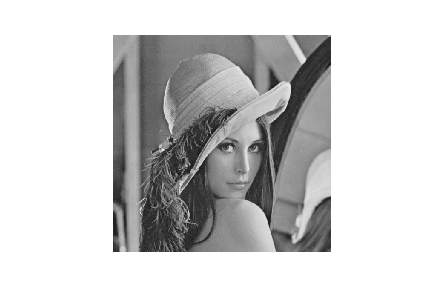
\includegraphics[width=8.5cm]{Figures/lena_rect_filter}}
		%  \vspace{2.0cm}
		\centerline{Lena com filtro de média retangular 5x5 aplicado.}\medskip
	\end{minipage}
\end{figure}

O algoritmo construído para gerar a esse resultado pode ser encontrado na Figura \ref{fig:rect_filter_lena}.

\subsection*{2.c - Unsharp Masking}

\textit{Unsharp masking} é um processo que visa aumentar a nitidez da imagem e pode ser dividido em alguns passos:

\begin{enumerate}
	\item Borrar a imagem original (como feito na questão anterior, por exemplo);
	\item Subtrair da imagem original a imagem borrada, gerando a máscara;
	\item Adicionar a máscara à imagem original.
\end{enumerate}

Para realizar esse processo, implementou-se o código \ref{cod:unsharp_mask}

\subsection*{2.d - High Boost}
O \textit{High boost} é o nome dado quando utiliza-se da técnica de \textit{unsharp masking} com diferente fatores multiplicativos. Ou seja, ao invés de apenas adicionar a máscara novamente no passo 4, multiplica-se a máscara por determinados fatores para depois somá-la à imagem.

A implementação dessa técnica está descrita no Código \ref{cod:high_boost}

\subsection*{2.e - Imagens sem escalonamento}
Utilizando os códigos \ref{cod:unsharp_mask} e \ref{cod:high_boost} e aplicando-os nas imagens com \lstinline{scaled = False}, obtemos os seguintes resultados:

\begin{figure}[H]
	\label{fig:lena_mask_without_scalling}
	\begin{minipage}[b]{1.0\linewidth}
		\centering
		\centerline{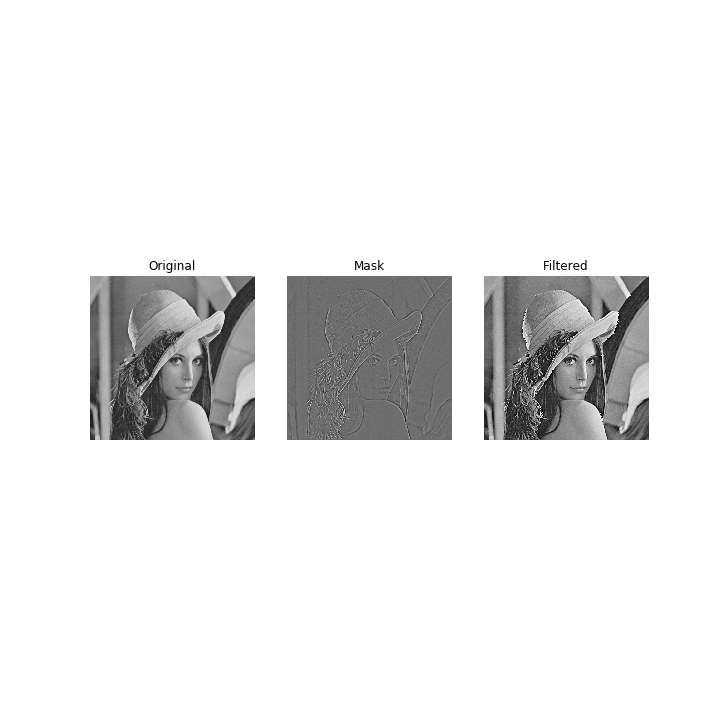
\includegraphics[width=8.5cm]{Figures/unsharp_mask_without_scalling}}
		%  \vspace{2.0cm}
		Lena com a técnica de Unsharp Masking aplicada sem escalonamento.\medskip
	\end{minipage}
\end{figure}

\begin{figure}[H]
	\label{fig:lena_boost_without_scalling}
	\begin{minipage}[b]{1.0\linewidth}
		\centering
		\centerline{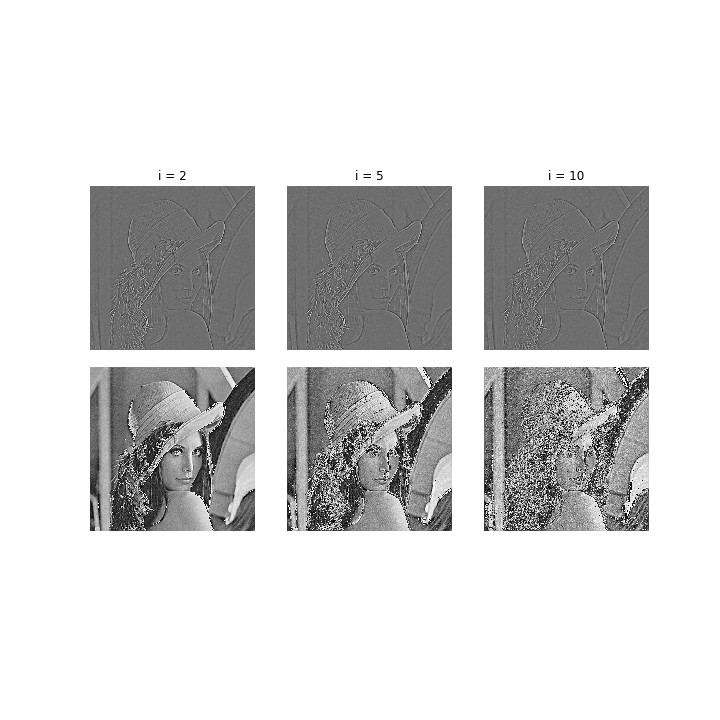
\includegraphics[width=8.5cm]{Figures/high_boost_without_scalling}}
		%  \vspace{2.0cm}
		Lena com a técnica de High Boost aplicada (k = 2, 5 e 10) sem escalonamento.\medskip
	\end{minipage}
\end{figure}


\subsection*{2.f - Aplicando o escalonamento desenvolvido}

\begin{figure}[H]
	\label{fig:lena_mask_with_scalling}
	\begin{minipage}[b]{1.0\linewidth}
		\centering
		\centerline{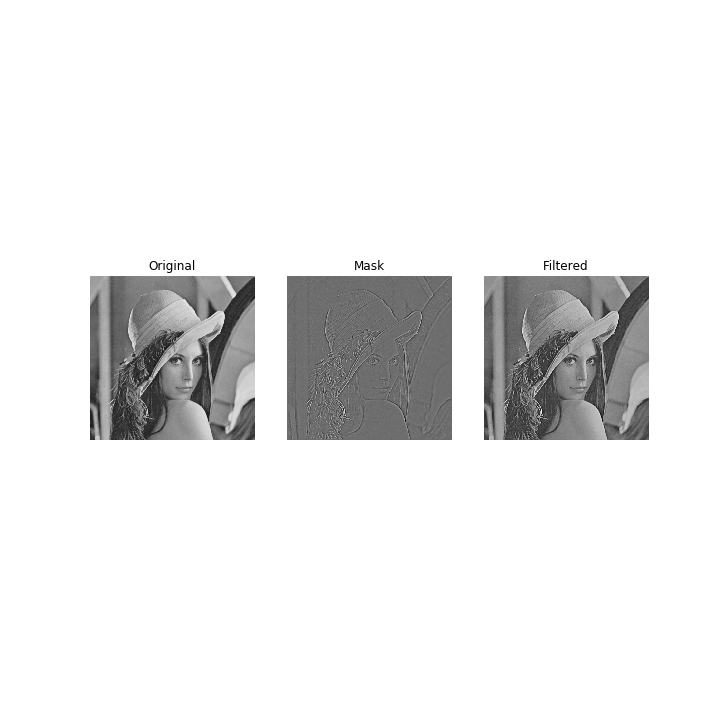
\includegraphics[width=8.5cm]{Figures/unsharp_mask_with_scalling}}
		%  \vspace{2.0cm}
		Lena com a técnica de Unsharp Masking aplicada com escalonamento.\medskip
	\end{minipage}
\end{figure}

\begin{figure}[H]
	\label{fig:lena_boost_with_scalling}
	\begin{minipage}[b]{1.0\linewidth}
		\centering
		\centerline{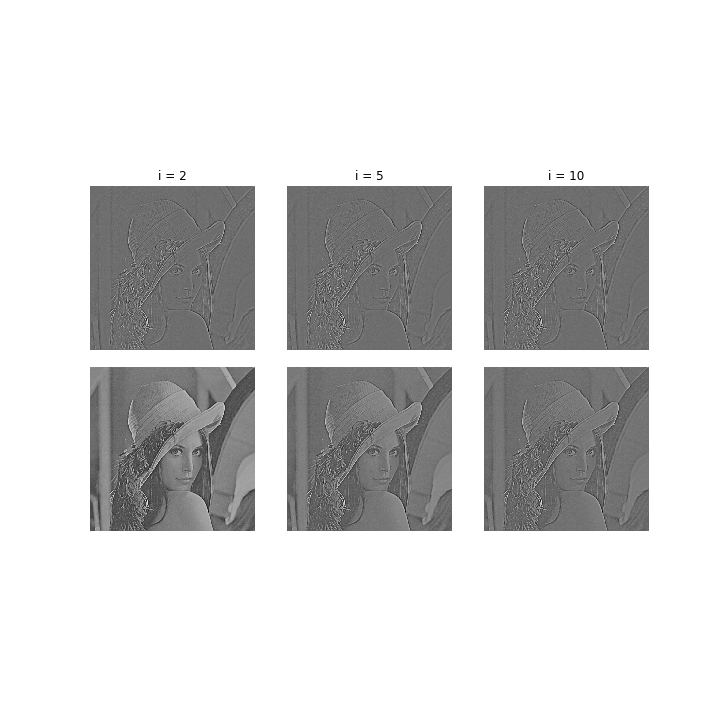
\includegraphics[width=8.5cm]{Figures/high_boost_with_scalling}}
		%  \vspace{2.0cm}
		Lena com a técnica de High Boost aplicada (k = 2, 5 e 10) com escalonamento.\medskip
	\end{minipage}
\end{figure}
\newpage
\subsection*{2.g - Discussão}	

Olhando para as imagens geradas com e sem escalonamento obtidas no exercício anterior, torna-se possível fazer algumas análises sobre suas características e suas diferenças:

\begin{enumerate}
	\item As imagens escalonadas estão com um nível muito elevado de níveis de cinza;
	\item Nas imagens nas quais não não foi aplicado o escalonamento, quanto mais elevado é o fator multiplicativo, maior é o número de artefatos que a imagem resultante tem;
\end{enumerate}

Fazendo uma análise nos valores obtidas, notou-se que se removermos os valores que ultrapassam os limites do uint8, ou seja, valores menores que zero e maiores que 255, esses artefatos da imagem não escalonada se tornam significantemente menores, melhorando muito a qualidade e a visualização da imagem.

Isso acontece porque o método utilizado para conversão (\lstinline|np.ndarray.astype()|) realiza um processo diferente para a adequação desses valores à faixa requerida pelo tipo de variável especificado (no nosso caso, valores entre 0 e 255, totalizando 256 níveis de cinza).

\textbf{Ex.:} Se nós tivermos um pixel de valor \lstinline|pixel = -30| e usarmos algo do tipo \lstinline|new_pixel = pixel.astype(np.uint8)|, o resultado será calculado como \lstinline|256 - 30 = 226|. Similarmente, se tivermos um outro valor \lstinline|pixel = 400|, após aplicarmos o mesmo procedimento o valor do pixel resultante será \lstinline|400 - 256 = 144|.

Os resultados discutidos podem ser melhor visualizados nas figuras a seguir.

\begin{figure}[H]
	\label{fig:lena_mask_cut}
	\begin{minipage}[b]{1.0\linewidth}
		\centering
		\centerline{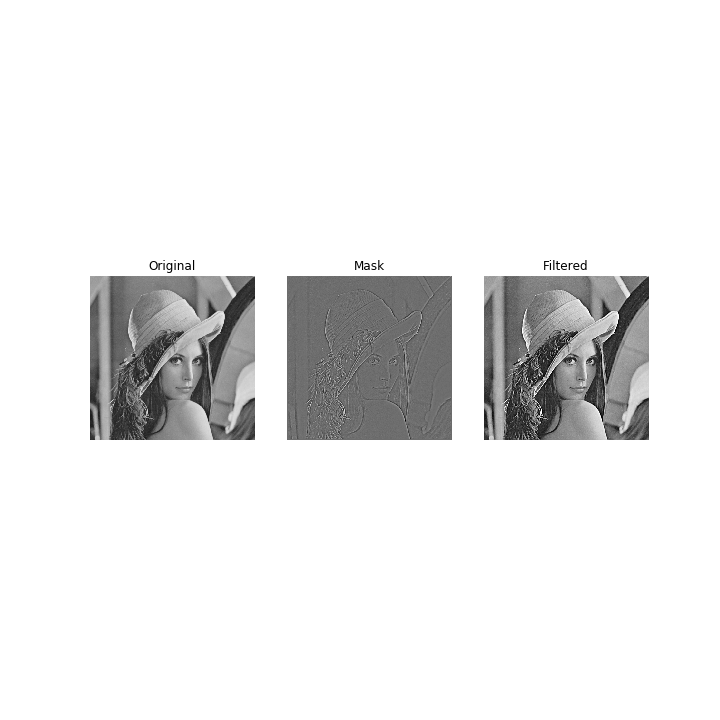
\includegraphics[width=8.5cm]{Figures/cutted_unsharp_mask}}
		%  \vspace{2.0cm}
		Lena com a técnica de Unsharp Masking aplicada  com valores cortados.\medskip
	\end{minipage}
\end{figure}

\begin{figure}[H]
	\label{fig:lena_boost_cut}
	\begin{minipage}[b]{1.0\linewidth}
		\centering
		\centerline{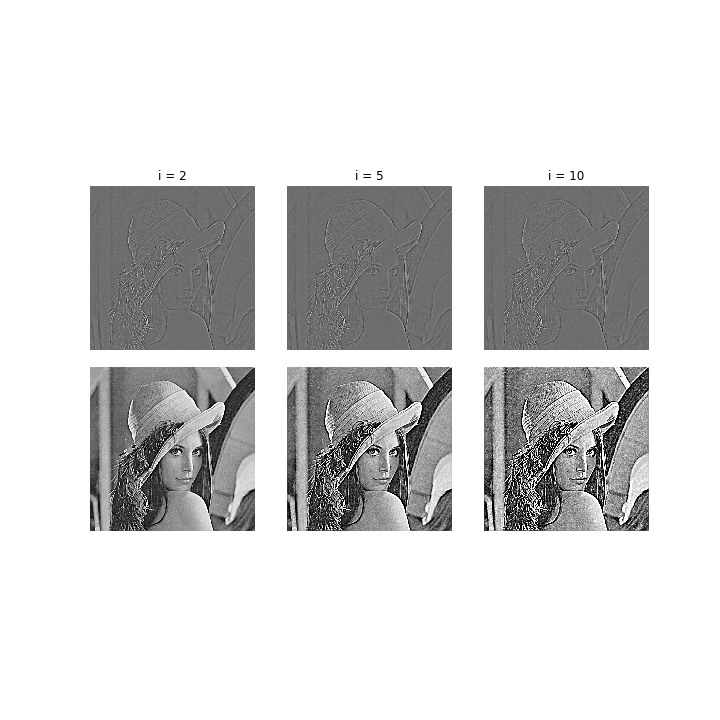
\includegraphics[width=8.5cm]{Figures/cutted_high_boost}}
		%  \vspace{2.0cm}
		Lena com a técnica de High Boost aplicada (k = 2, 5 e 10) com os valores cortados.\medskip
	\end{minipage}
\end{figure}


Com relação às imagens escalonadas, que passam a possuir valores com níveis de cinza similares em sua composição, deve-se ao fato de os pixels da máscara possuírem valores muito mais altos de intensidade. Com isso, depois de escalonada, os intervalos entre os pixels da imagem se tornam muito menores, para que o espaço de 256 valores seja capaz de suportar os valores mais altos e mais baixos da máscara. Deve-se considerar ainda o fato de que, na técnica do high boost, os valores da máscara foram multiplicados em até 10 vezes, aumentando ainda mais essa discrepância. 

% To start a new column (but not a new page) and help balance the last-page
% column length use \vfill\pagebreak.
% -------------------------------------------------------------------------
%\vfill
%\pagebreak
\newpage
\onecolumn
\section{Códigos}

\subsection{Geração do histograma da imagem}
\label{cod:hist}
\begin{python}
def my_histogram(image, plot = True, amax = 256, norm = False):
	if(len(image.shape) > 2):
	image = cv2.cvtColor(image, cv2.COLOR\_BGR2GRAY)
	
	# Get number of lines and columns
	qntI, qntJ = image.shape
	
	# Creating Histogram manually
	histogram = np.zeros(amax)
	color = 0
	for i in range(qntI):
		for j in range(qntJ):
			color = image[i][j]
			\# print(color)
			histogram[color] += 1
	
	if(norm):
		histogram = (histogram - np.amin(histogram)) /  (np.amax(histogram) - np.amin(histogram))
	
	if(plot):
		plt.figure()
		plt.stem(histogram, use\_line\_collection = True)
		plt.title('Original Image Histogram \$p\_r(r)\$')
		plt.show()
	return histogram
\end{python}

\newpage

\subsection{Geração da CDF a partir do histograma}
\label{cod:cdf_2d}
\begin{python}
def cdf_2D(img, plot = True, amax = 256, norm = False):
	cdf = np.zeros(amax)

	if(len(img.shape) > 2):
		img = cv2.cvtColor(img, cv2.COLOR_BGR2GRAY)
	
	# Get number of lines and columns
	qntI, qntJ = img.shape
	
	# Number of pixels
	qnt_pixels = qntI * qntJ
	
	histogram = my_histogram(img, amax = amax, norm = norm, plot = False)
	
	# print(len(histogram))
	for h in range(amax):
		cdf[h] = np.sum(histogram[0: h + 1]) / qnt_pixels 
	
	if(plot):
		plt.figure()
		plt.stem(cdf, use_line_collection = True)
		plt.plot(cdf, 'k')
		plt.title('Cumulative Distribution Function (CDF) $G(s)$')
		plt.show()
	return cdf
\end{python}

\newpage

\subsection{Geração da CDF a partir da PDF}
\label{cod:cdf_pdf}
\begin{python}
def cdf_pdf(pdf, plot = True):
	cdf = np.zeros(len(pdf))
	for h in range(len(pdf)):
		cdf[h] = np.sum(pdf[0: h + 1])
		
	if(plot):
		plt.figure()
		plt.stem(pdf, use_line_collection = True)
		plt.title('Probability Density function (PDF) $p_z(z)$')
		plt.show()
		
		plt.figure()
		plt.stem(cdf, use_line_collection = True)
		plt.plot(cdf, 'k')
		plt.title('Cumulative Distribution Function (CDF) $G(z)$')
		plt.show()
	return cdf	

\end{python}

\newpage
\subsection{Transformação inversa}
\label{cod:inv_t}
\begin{python}
def inv_cdf(img, required_pdf, amax = 256):
	if(len(img.shape) > 2):
		img = cv2.cvtColor(img, cv2.COLOR_BGR2GRAY)
		
	x, y = img.shape
	new_img = img
	
	s = np.round(np.multiply((amax - 1), cdf_2D(img, plot = False)))
	G = np.round(np.multiply((amax - 1), cdf_pdf(required_pdf, plot = False)))
	
	s = s.astype(np.uint8)
	new_z = np.zeros(amax)
	G_s = np.zeros(amax)
	diffs = []
	
	for k in range(amax):
		diffs = np.abs(np.subtract(G, s[k]))
		new_z[k] = np.argmin(diffs)
		G_s[s[k]] = np.argmin(diffs)
	
	plt.figure()
	plt.stem(G, linefmt = 'k', use_line_collection = True)
	plt.plot(s, '-or')
	plt.legend(['$s_k$', '$G(z_k)$'])
	plt.show()
	
	plt.figure()
	markerline, stemlines, baseline = plt.stem(s, G_s[s], linefmt = 'k', markerfmt = '-oc', use_line_collection = True)
	plt.setp(baseline, color='k', linewidth=2)
	plt.setp(markerline, linewidth=3)
	plt.title('Mapping s in z')
	plt.xlabel('original values (s)')
	plt.ylabel('new values ($z = G^{-1}(s)$)')
	plt.show()
	
	for i in range(x):
		for j in range(y):
			new_img[i][j] = new_z[img[i][j]]
	new_img = new_img.astype(np.uint8)
return new_img
\end{python}

\newpage
\subsubsection{Conversão de Imagens em float para inteiro}
\label{cod:linear}
\begin{python}
def rescale(xmax, xmin, ymax, ymin):
	a = (ymax - ymin) / (xmax - xmin)
	b = ((ymin * xmax) - (ymax * xmin)) / (xmax - xmin) 
	return a, b

def img2int(img):
	img_max = img.max()
	img_min = img.min()
	
	int_max = 255
	int_min = 0
	
	a, b = rescale(img_max, img_min, int_max, int_min)
	rescaled_img = np.multiply(a, img) + b
	return rescaled_img.astype(np.uint8)
\end{python}

\newpage
\subsubsection{Unsharp Masking}
\label{cod:unsharp_mask}
\begin{python}
from skimage.filters import unsharp_mask

def unsharpe_masking(img, blurry_img, scaled = True, method = 'myMethod', plot = True, cut_out = False):
	if(len(img.shape) > 2):
		img = cv2.cvtColor(img, cv2.COLOR_BGR2GRAY)
	
	if(method is 'myMethod'):
		img = img.astype(np.float)
		blurry_img = blurry_img.astype(np.float)
		
		mask = np.subtract(img, blurry_img)
		new_img = np.array(mask) + np.array(img)
		if(cut_out):
			new_img[new_img < 0] = 0
			new_img[new_img > 255] = 255
		if(scaled):
			new_img = img2int(new_img)
		new_img = new_img.astype(np.uint8)
		
		if(plot):
			plt.figure()
			fig, axs = plt.subplots(1, 3, figsize = (10, 10))
			axs[0].imshow(img, cmap = 'gray', vmin = 0, vmax = 255)
			axs[1].imshow(mask, cmap = 'gray')
			axs[2].imshow(new_img, cmap = 'gray', vmin = 0, vmax = 255)
			
			axs[0].axis('off')
			axs[1].axis('off')
			axs[2].axis('off')
			
			axs[0].title.set_text('Original')
			axs[1].title.set_text('Mask')
			axs[2].title.set_text('Filtered')
	
		elif(method is 'skimage'):
			new_img = unsharp_mask(img, radius=1, amount=1) * 255
			new_img = new_img.astype(np.uint8)
	
			if(plot):
				plt.figure()
				fig, axs = plt.subplots(1, 2, figsize = (10, 10))
				axs[0].imshow(img, cmap = 'gray', vmin = 0, vmax = 255)
				axs[1].imshow(new_img, cmap = 'gray', vmin = 0, vmax = 255)
				
				axs[0].axis('off')
				axs[1].axis('off')
				if(plot):
				plt.subplots_adjust(hspace = - 0.5)
				plt.show()
				
	return new_img
\end{python}

\newpage
\subsubsection{Unsharp Masking}
\label{cod:high_boost}
\begin{python}
def high_boost(img, blurry_img, k = [2, 5, 10], scaled = True, method = 'myMethod', plot = True, cut_out = False):
	if(len(img.shape) > 2):
		img = cv2.cvtColor(img, cv2.COLOR_BGR2GRAY)
	new_img = {}
	f = 0
	
	if(plot):
		n_figs = (2 * len(k))
		m = 2
		n = int(n_figs / m)
		plt.figure()
		fig, axs = plt.subplots(m, n, figsize = (10, 10))
		# axs[f].imshow(img, cmap = 'gray')
	
	if(method is 'myMethod'):
	img = img.astype(np.float)
	blurry_img = blurry_img.astype(np.float)
	for i in k:
		mask = np.multiply(np.subtract(img, blurry_img), i)
		new_img[f] = np.array(mask) + np.array(img)
	
		if(cut_out):
			new_img[f][new_img[f] < 0] = 0
			new_img[f][new_img[f] > 255] = 255
			
		if(scaled):
			new_img[f] = img2int(new_img[f])
			
		new_img[f] = new_img[f].astype(np.uint8)
		
		if(plot):
			axs[0][f].imshow(mask, cmap = 'gray')
			axs[0][f].title.set_text('i = %d' % i)
			axs[1][f].imshow(new_img[f], cmap = 'gray', vmin = 0, vmax = 255)
			axs[0][f].axis('off')
			axs[1][f].axis('off')
			plt.subplots_adjust(hspace = - 0.5)
		
		f = f + 1
	
	elif(method is 'skimage'):
		for i in k:
			new_img[f] = unsharp_mask(img, radius=1, amount=i) * 255
			print(new_img[f].min(), ', ', new_img[f].max())
			new_img[f] = new_img[f].astype(np.uint8)
			
		if(plot):
			axs[0][f].imshow(img, cmap = 'gray', vmin = 0, vmax = 255)
			axs[0][f].title.set_text('i = %d' % i)
			axs[1][f].imshow(new_img[f], cmap = 'gray', vmin = 0, vmax = 255)
			axs[0][f].axis('off')
			axs[1][f].axis('off')
			plt.subplots_adjust(hspace = - 0.5)
			
		f = f + 1
	if(plot):
		plt.show()
		
	return new_img
\end{python}

\end{document}
